% set 0.5 inch indentation
\setlength{\parindent}{0.5in} 
% set paragraph space = 0 space
\setlength{\parskip}{0mm}
% set line space 1.5
\setlength{\baselineskip}{1.6em}

\chapter{EXPERIMENTAL RESULTS}
\label{ch:results}
\textit{In this chapter, I run four experiments comprising three simulations with one, two and three drones and a real world experiment with one drone.  }

\section{Real World Experiment}
To test the automated system, an experiment is run in the Energy Park behind CSIM building. The site is chosen as it has structures which will help SURF descriptors recognize features. 
\subsubsection{Mesh Network}

The mesh network consists of two wireless mesh routers running OpenWrt. Both of the routers are dual channel 2.5/5 GHz's routers with two radios. The GCS wireless router is a Netgear router (Figure~\ref{fig:gcs-router}). The GCS laptop is connected to the router via 2.5GHz WiFi network with SSID UAV01\_01. The TP-Link mobile wireless router (Figure~\ref{fig:mobile-router}) mounted on the drone is connected to the companion Raspberry Pi via Ethernet. The SSID of the mesh network is UAV01\_MESH5G and is running on 5 GHz channel. Figure~\ref{fig:mesh-network-real-world} shows the network infrastructure used.

The GCS laptop and companion are not mesh clients but are connected to different networks. Route between the GCS laptop and companion Raspberry Pi is achieved by using OSLR Host and network association (HNA) message to allow connection to these networks. Since GCS laptop is connected to different subnet than the Raspberry Pi, a route \texttt{\$ sudo route add -net 192.168.41.0/24 gw 192.168.40.1 wlp0s20f3} has to be added manually in the GCS laptop to divert the packet for the Raspberry Pi's subnet via the wireless LAN interface of the GCS to the the mesh network.

The IP assignment for different nodes in the network is given in Table~\ref{tab:network-assignment}.


\begin{table}[t]
	\caption[IP assignment for real world experiment]{\small IP assignment for real world experiment}
	\begin{center}
		\begin{tabular}{c|c|c|c}
			\hline Node & IP Address & Subnet & OSLR Interface IP\\ \hline \hline
			GCS Wireless Router & 192.168.40.1 &  192.168.40.1/24 & 192.168.30.1 \\ \hline
			Mobile Wireless Router & 192.168.41.1 & 192.168.41.1/24 & 192.168.30.2   \\ \hline 
			GCS Laptop & 192.168.40.216 & 192.168.40.1/24 & -  \\ \hline 
			Companion Raspberry Pi & 192.168.41.200 & 192.168.41.1/24 & - \\ \hline
		\end{tabular}
	\end{center}
	\label{tab:network-assignment}
\end{table} 


\begin{figure}
	\centering
	\caption[Network infrastructure for real world experiment]{\small Network infrastructure for real world experiment.} 
	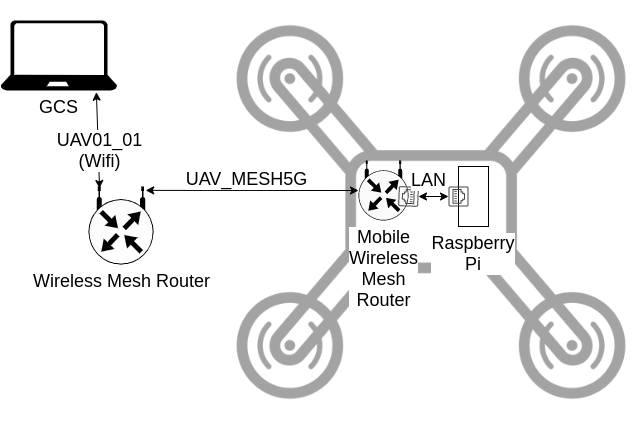
\includegraphics[width=5in]{figures/experiment/real-world-network}
	\label{fig:mesh-network-real-world}
\end{figure}

\begin{figure}
	\centering
	\caption[Wireless routers used in experiment.]{\small 
		(a) Netgear wireless router for the GCS. (b) TP-Link mobile wireless router mounted on the drone. }
	\subfloat[]{%
		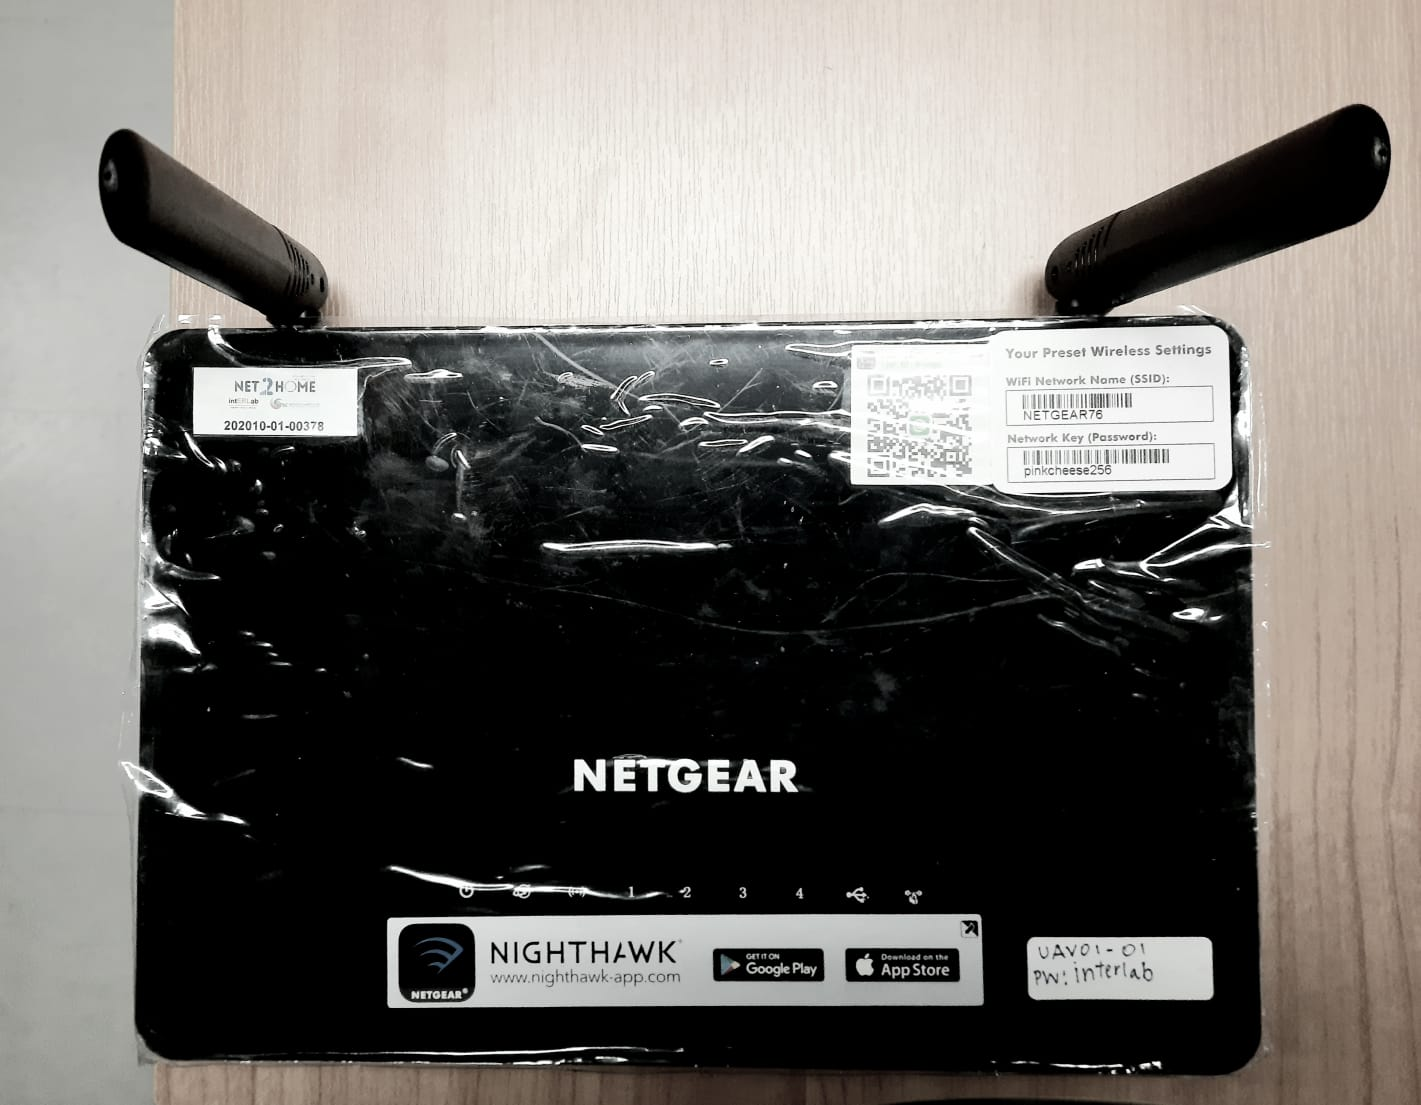
\includegraphics[width=3in]{figures/experiment/router2-mesh}
		\label{fig:gcs-router}
	}
	\subfloat[]{%
		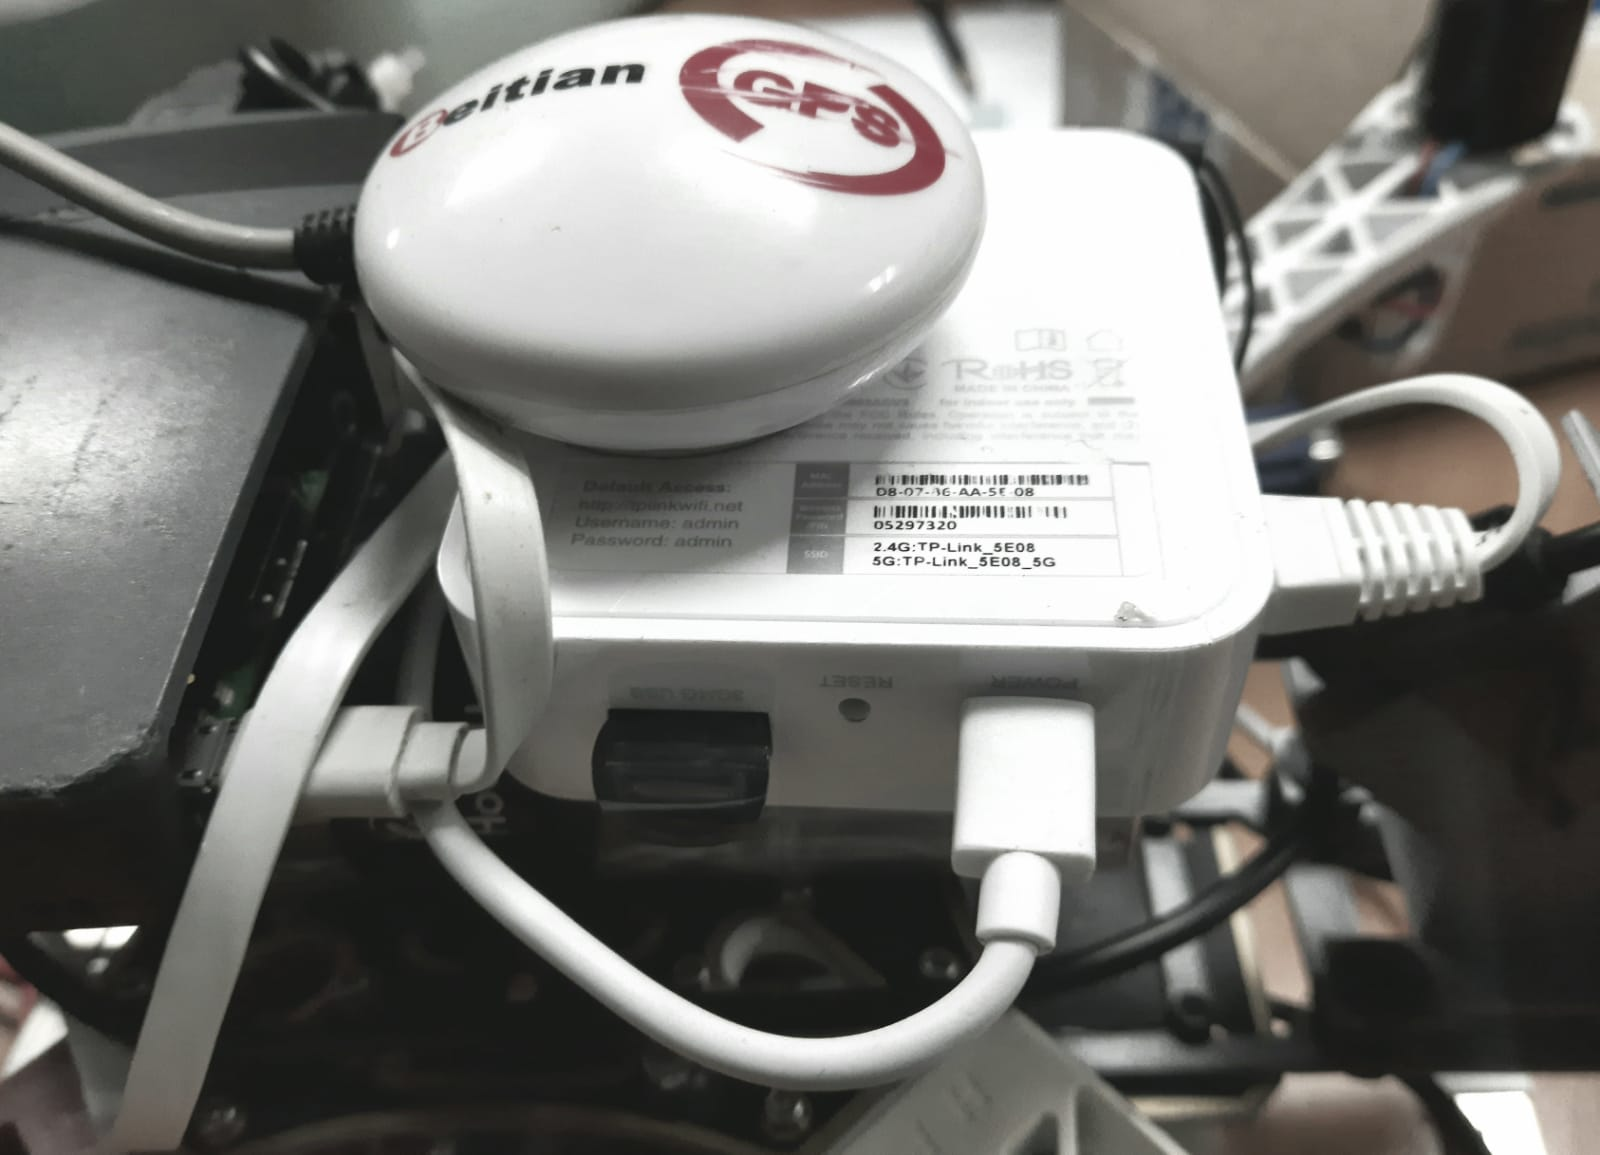
\includegraphics[width=3in]{figures/experiment/router1-mesh}%
		\label{fig:mobile-router}
	}
	
	\label{fig:real-routers}
\end{figure}

\subsection{Automated Planning}

For planning the path, the operational altitude is set at 20 meters, the grid size is set at 10 meters and the mesh range is set at 40 meters. The results of planning is given in Table~\ref{tab:real-world-planning}. The viewpoints and the path generated is shown is Figure~\ref{fig:real-path}.
\begin{table}[t]
	\caption[Result of \texttt{pegasus\_planner} in real world experiment.]{\small Result of\texttt{pegasus\_planner} in real world experiment.}
	\begin{center}
		\begin{tabular}{c|c|c|c}
			\hline Type & Number of Drones & Viewpoints Generated & Path Size \\ \hline \hline
			Real Experiment & 1 & 16 & 18 \\ \hline
		\end{tabular}
	\end{center}
	\label{tab:real-world-planning}
\end{table} 


\begin{figure}
	\centering
	\caption[Path generated for real world experiment.]{\small Path generated for real world experiment.} 
	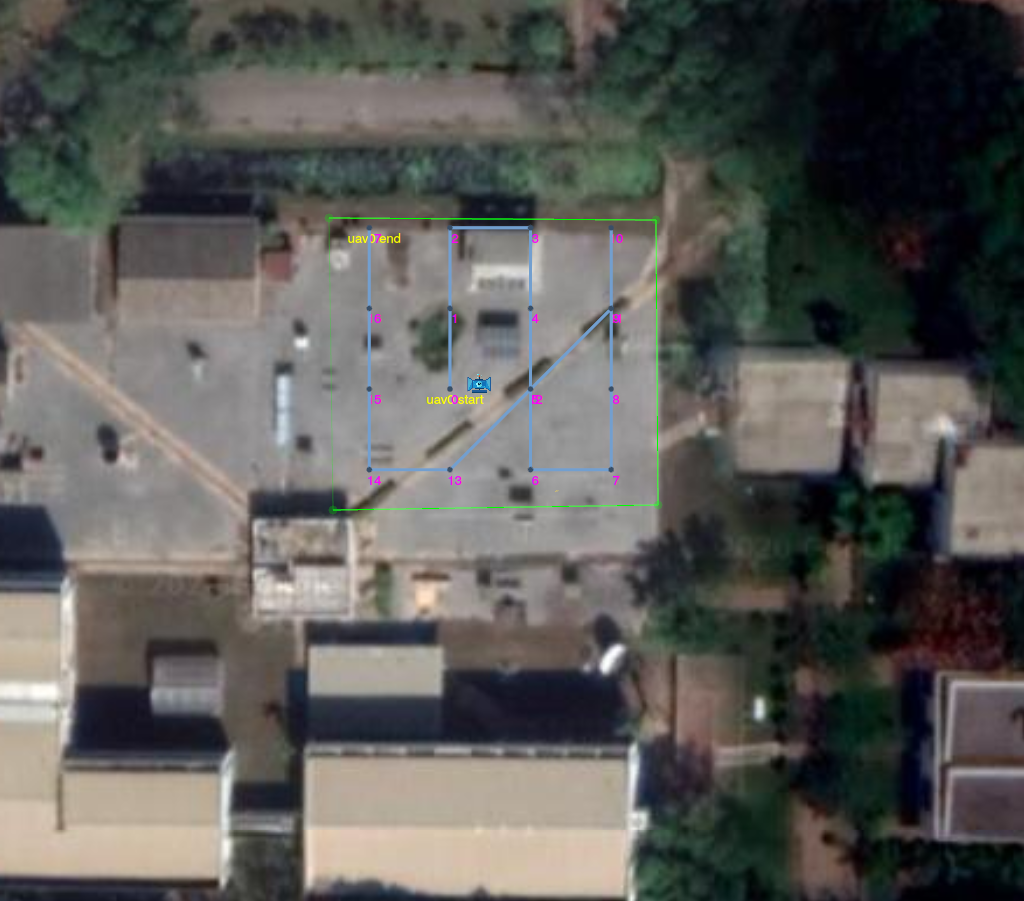
\includegraphics[width=5in]{figures/experiment/real_mapviz_plan}
	\label{fig:real-path}
\end{figure}

\subsection{Motion Control}
The pegasus\_controller was able to successfully communicate with the pegasus\_commander in the drone and control the motion of the drone in off-board mode throughout the experiment. The movement type was set to strafe to reduce the time taken for the mission as the drone would not need to align itself at yaw 0\degree after reaching each viewpoint. The pegasus\_controller was successfully able to calculate the transform between the local map of the drone and the global map after the calibration routine. To ensure the safety of the drone, the system was started with the drone in HOLD mode at 20 meters altitude. There was a slight drift in the position of the drone when it was being set to off-board mode through the companion computer. The actual path of the drone during the mission as reported by GPS data received through the heart beat reply is shown in Figure~\ref{fig:real-gps}. The figure does not show drone returning to its home position after the end of the mission because heart beat message is stopped after the drone has reached and collected image in the last pose of its path. Figure~\ref{fig:q-real-gps} shows the complete mission path in QGroundControl.


\begin{figure}
	\centering
	\caption[GPS position reported through pegasus system.]{\small GPS position reported through pegasus system.} 
	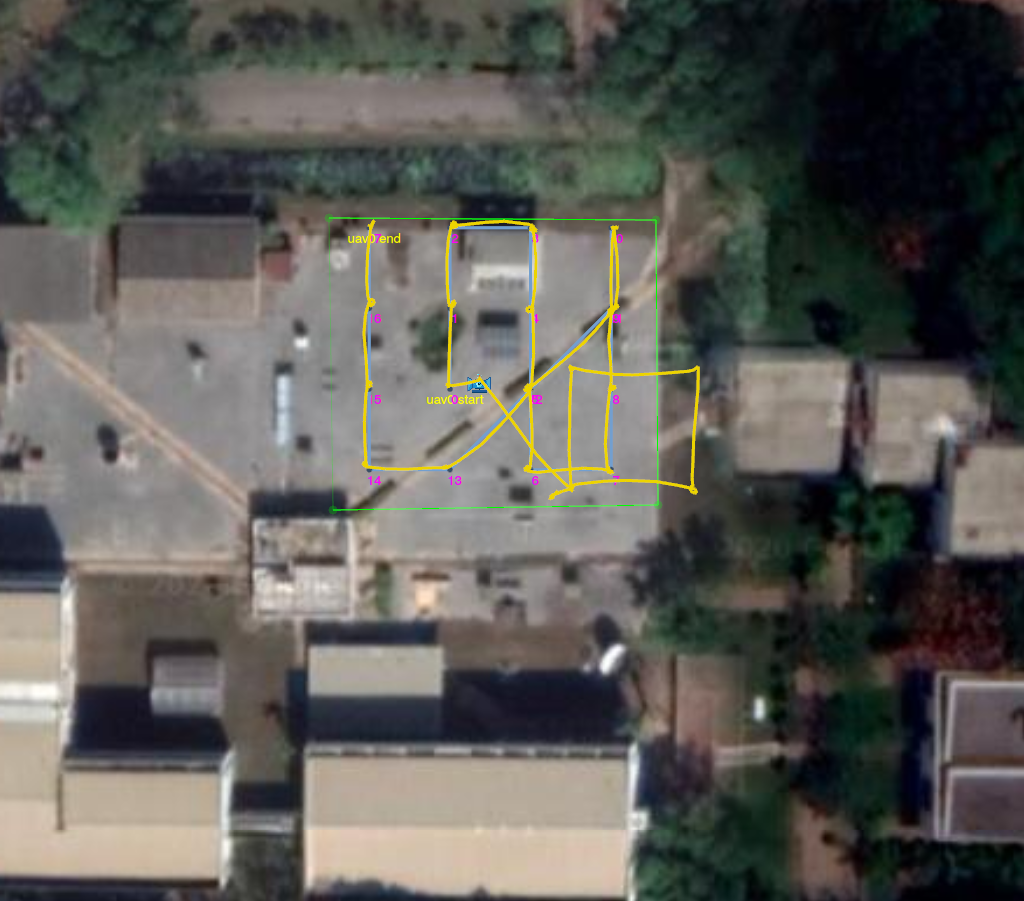
\includegraphics[width=5in]{figures/experiment/real_mapviz_path}
	\label{fig:real-gps}
\end{figure}

\begin{figure}
	\centering
	\caption[GPS position reported through telemetry wifi.]{\small GPS position reported through telemetry WiFi in QGroundControl.} 
	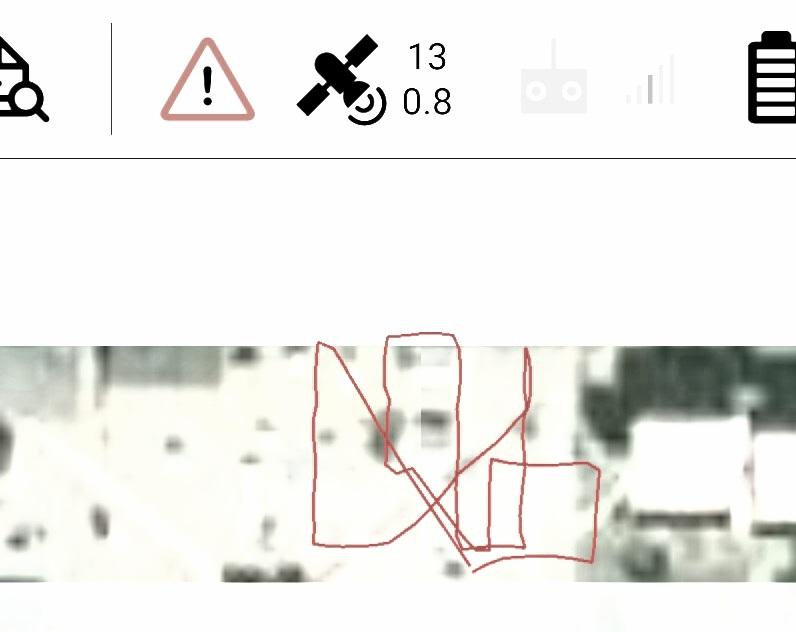
\includegraphics[width=5in]{figures/experiment/q-ground-control}
	\label{fig:q-real-gps}
\end{figure}


\subsection{Images Captured}

The pegasus\_image\_subscriber and pegasus\_image\_publisher successfully acquired 16 images from 16 viewpoints in the mission in real-time as shown in Figure~\ref{fig:real-images}. Using an application called photini, the location of the images can be seen in Figure~\ref{fig:exif-real-images}. 
\begin{figure}
	\centering
	\caption[Images captured by pegasus in real-time.]{\small Images captured by pegasus in real-time.} 
	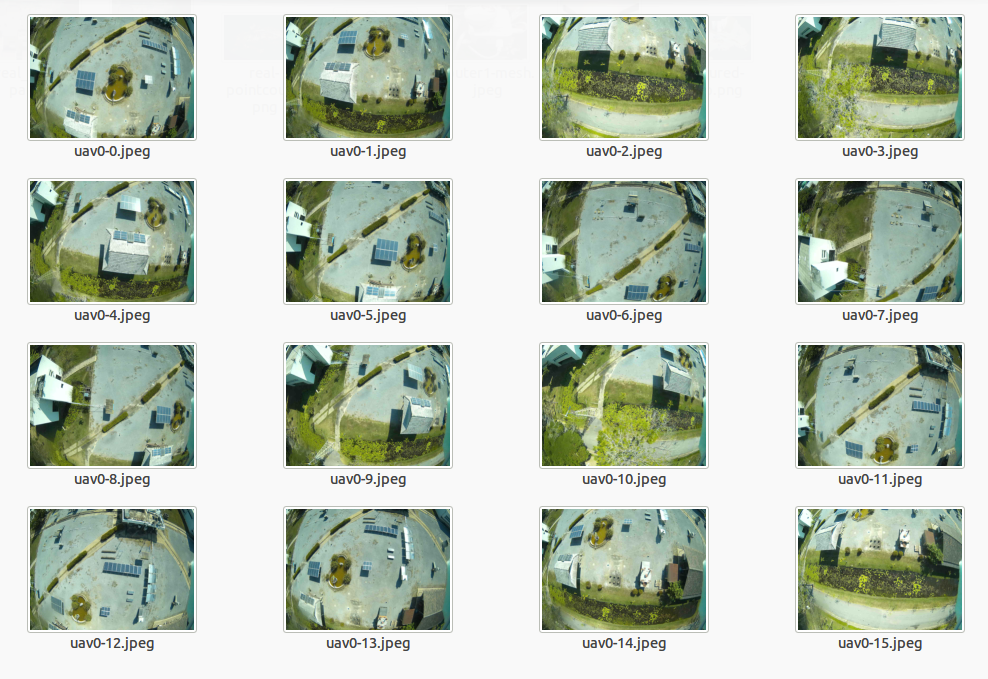
\includegraphics[width=6in]{figures/experiment/real-images}
	\label{fig:real-images}
\end{figure}

\begin{figure}
	\centering
	\caption[Location of images captured.]{\small Location of images captured.} 
	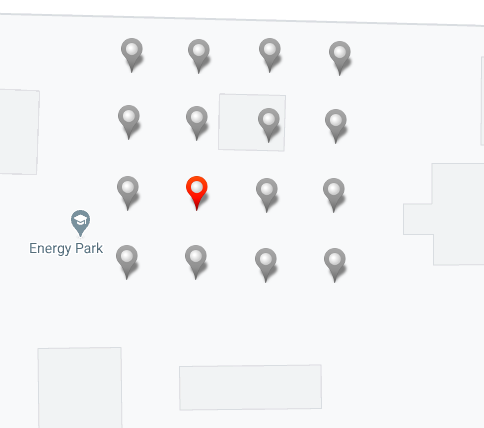
\includegraphics[width=5in]{figures/experiment/real-images-exif-tag}
	\label{fig:exif-real-images}
\end{figure}

\subsection{Result}
The images captured is rectified using pegasus\_image\_rectify using the camera calibration file. Then the rectified images are processed using WebODM.
\begin{itemize}
	\item Figure~\ref{fig:orthophoto-real} shows the orthophoto of the region of interest.
	\item Figure~\ref{fig:real-pointcloud} shows the point cloud of the region of interest.
	\item Figure~\ref{fig:real-textured-map} shows the textured model of the region of interest.
	\item Figure~\ref{fig:real-camera-position} shows the camera position as determined by ODM of the region of interest.
\end{itemize}

\begin{figure}
	\centering
	\caption[Orthophoto of Energy Park.]{\small Orthophoto of Energy Park.} 
	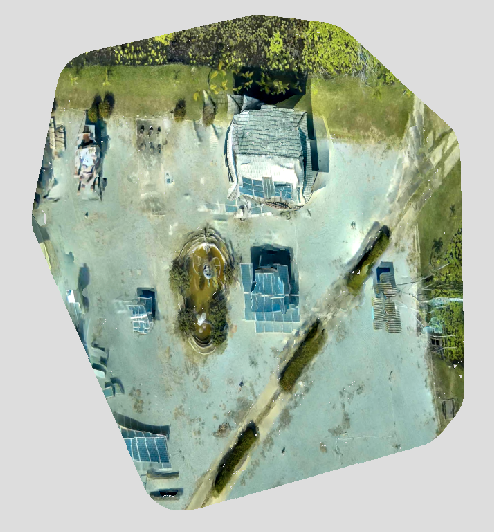
\includegraphics[width=5in]{figures/experiment/orthophoto-real}
	\label{fig:orthophoto-real}
\end{figure}

\begin{figure}
	\centering
	\caption[Point cloud of Energy Park.]{\small Point cloud of Energy Park.} 
	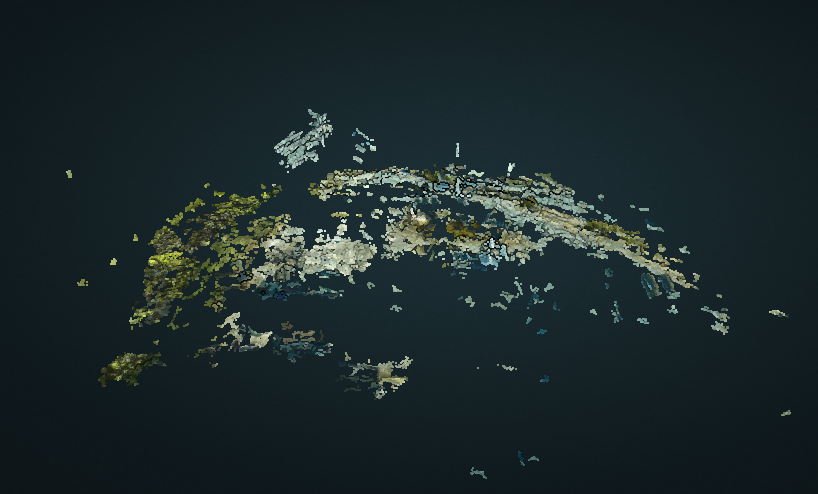
\includegraphics[width=5in]{figures/experiment/real-pointcloud}
	\label{fig:real-pointcloud}
\end{figure}

\begin{figure}
	\centering
	\caption[Textured mesh of Energy Park.]{\small Textured model of Energy Park.} 
	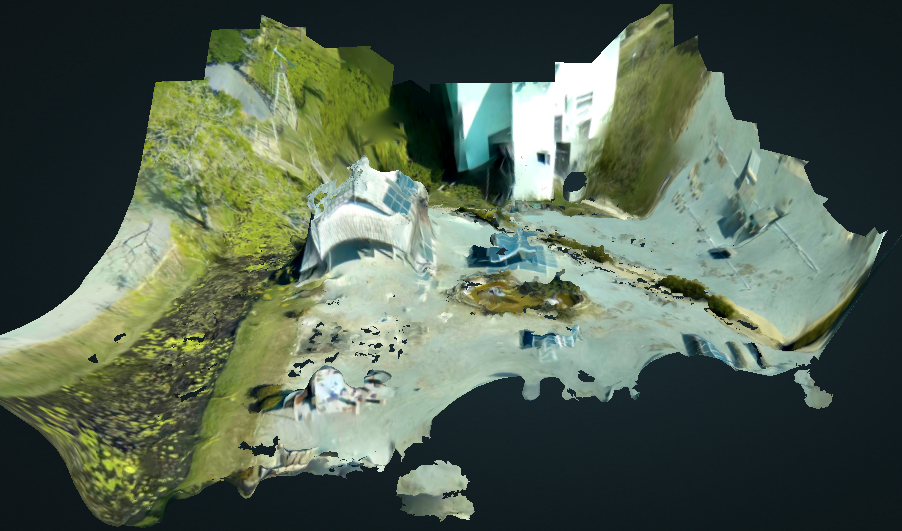
\includegraphics[width=5in]{figures/experiment/real-textured-map}
	\label{fig:real-textured-map}
\end{figure}

\begin{figure}
	\centering
	\caption[Camera Position calculated by ODM.]{\small Camera Position calculated by ODM.} 
	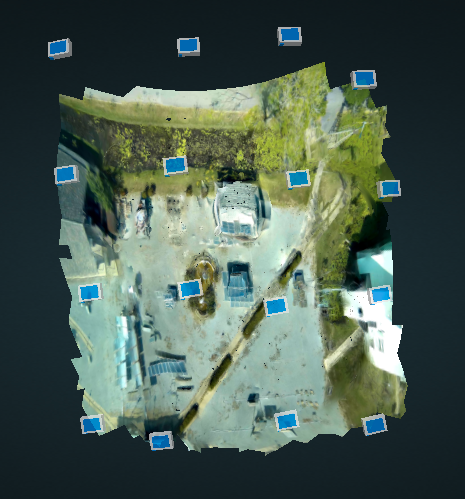
\includegraphics[width=5in]{figures/experiment/camera-position}
	\label{fig:real-camera-position}
\end{figure}

\section{Simulation}

Simulation will be run on the Gazebo world shown in Figure~\ref{fig:sim-world}. Simulation experiment will use 3 drones. 

\begin{figure}
	\centering
	\caption[Gazebo simulation world.]{\small Gazebo simulation world 
		(a) Top View. (b) Side View. }
	\subfloat[]{%
		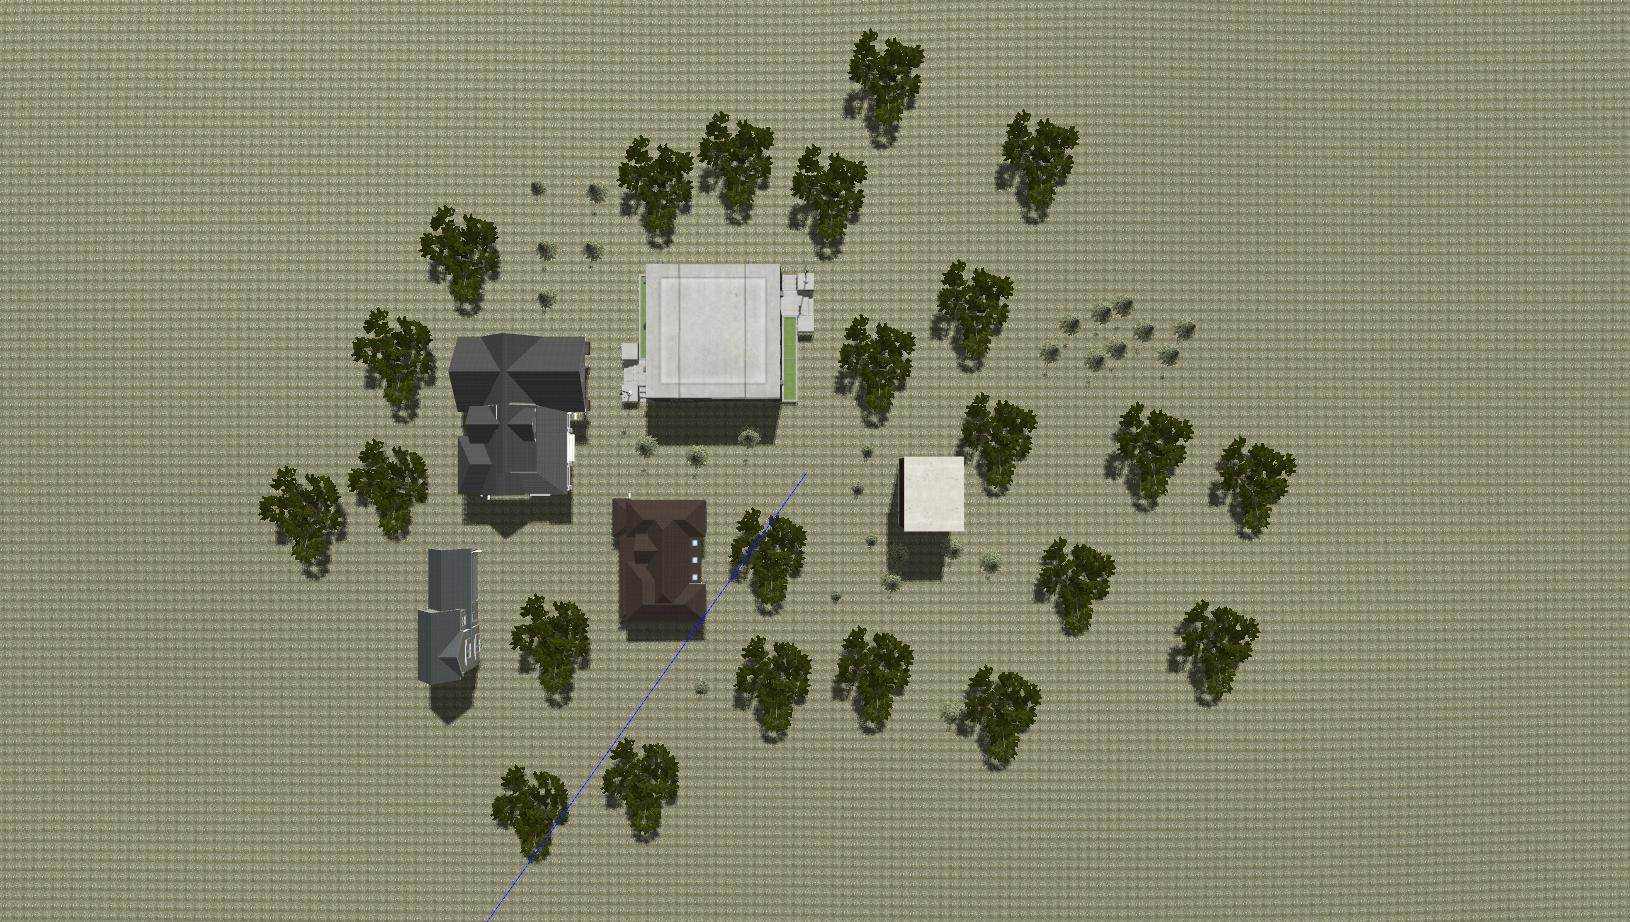
\includegraphics[width=5in]{figures/experiment/sim-world1}
	}
	
	\subfloat[]{%
		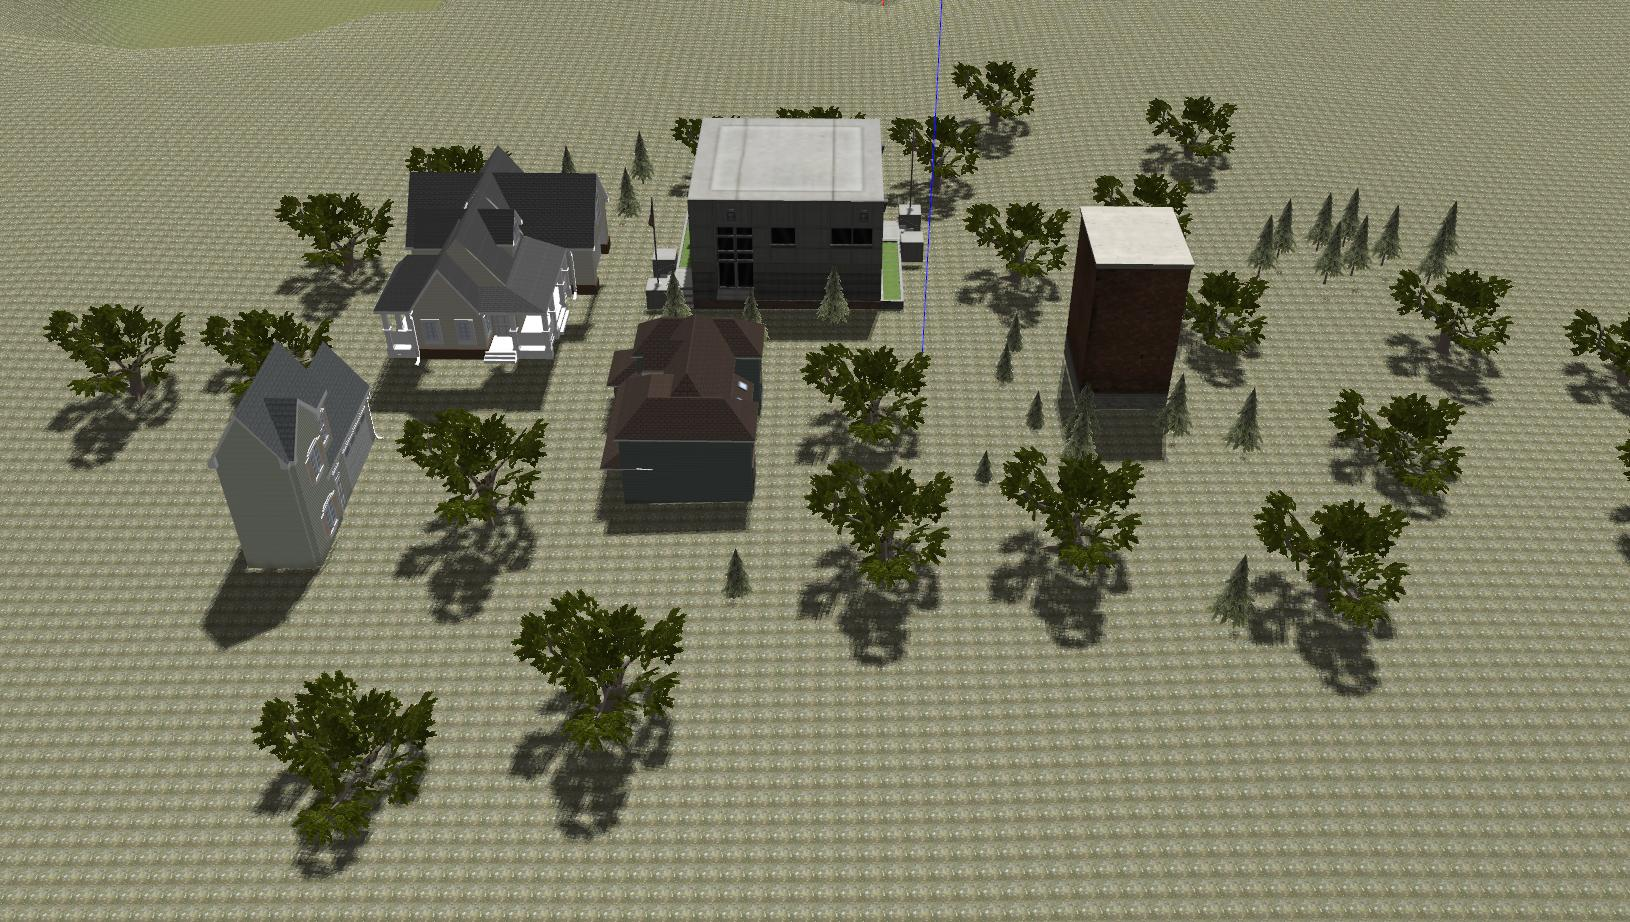
\includegraphics[width=5in]{figures/experiment/sim-world2}%
	}
	\label{fig:sim-world}
\end{figure}

\subsection{Simulated Network Configuration}

All the network packets will be routed though ns3. ns3 is configured with 3 drones each having a pegasus\_commander and pegasus\_controller. Therefore the GCS mush have a total of six udp sockets to control the system of three drones. The pegasus-net-sim ns3 simulator is configured as follows:

\begin{verbatim}
std::map<std::string, std::vector<PegasusPortConfig>> 
PegasusConfig::m_config {
{
"iris_0", {
{5444, 4444, 3444},
{7300, 7400, 7200},
}
},
{
"iris_1", {
{5445, 4445, 3445},
{7301, 7401, 7201},
}
},
{
"iris_2", {
{5446, 4446, 3446},
{7302, 7402, 7202},
}
},
{
CONTROL_STATION_STR , {
{3444, 6444, 5444},
{7200, 8200, 7300},
{3445, 6445, 5445},
{7201, 8201, 7301},
{3446, 6446, 5446},
{7202, 8202, 7302},
}
},
};
\end{verbatim}

\subsection{Automated Planning}
The area of interest is larger than the real world experiment with one drone and has more viewpoints. The operational height for the simulation is set at 30 meters. The grid size is set at 10 meters. The mesh range is set at 40 meters. The planning is completed at 3.74 seconds. The result of the planning is given in Table~\ref{tab:simulated-planning}. The path planned by the planner is shown in Figure~\ref{fig:simulated-plan}.

\begin{table}[t]
	\caption[Result of \texttt{pegasus\_planner} in simulated experiment with three drones.]{\small Result of \texttt{pegasus\_planner} in simulated experiment with three drones.}
	\begin{center}
		\begin{tabular}{c|c|c|c}
			\hline Type & Number of Drones & Viewpoints Generated & Path Size \\ \hline \hline
			Simulation & 3 & 25 & 11, 11, 10 \\ \hline
		\end{tabular}
	\end{center}
	\label{tab:simulated-planning}
\end{table}

\begin{figure}
	\centering
	\caption[Paths generated for three drones in simulation experiment.]{\small Paths generated for three drones in simulation experiment.} 
	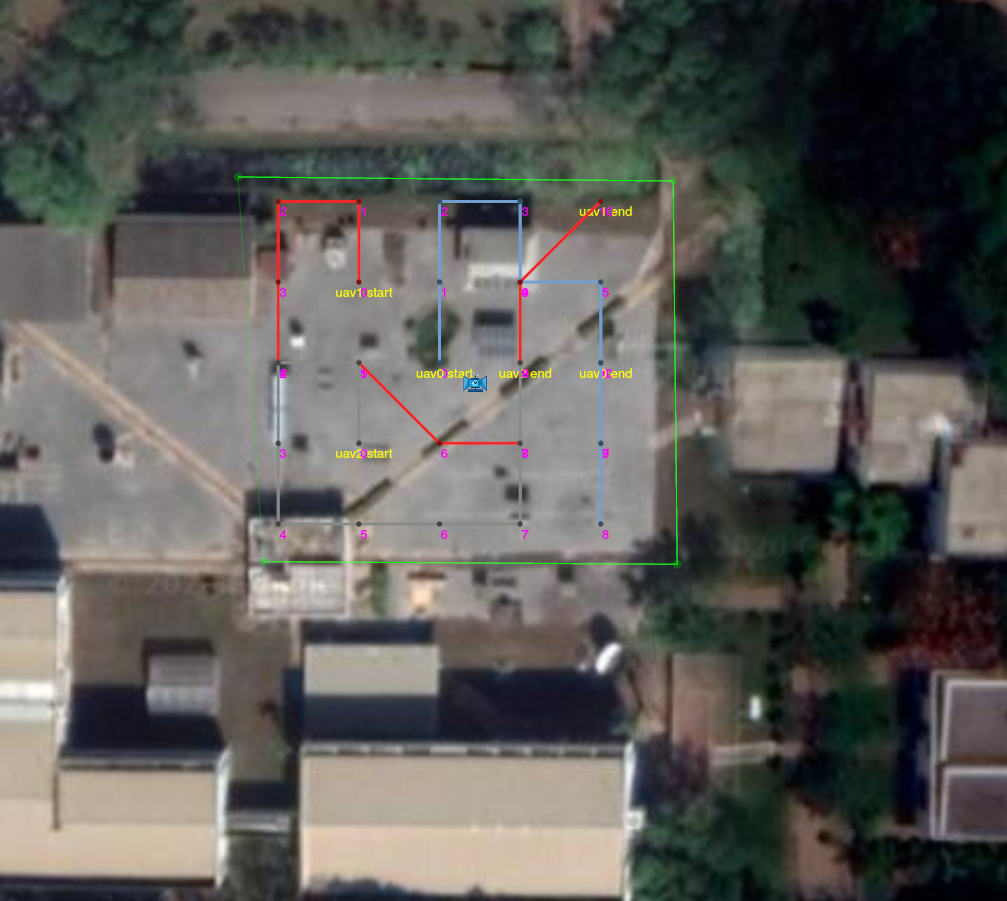
\includegraphics[width=5in]{figures/experiment/simulated-plan}
	\label{fig:simulated-plan}
\end{figure}

\subsection{Motion Control}
The pegasus\_controller is able to control three drones at once though pegasus\_commander in the drones. The transformation between the local maps of the drones and the global map is successfully calculated. pegasus\_controller is able to successfully carry out the coordinated mission without the drones colliding with each other.  The path taken by the drones are shown in Figure~\ref{fig:simulated-path}.

\begin{figure}
	\centering
	\caption[The path followed by the drones as reported through the simulated GPS of the drones.]{\small The path followed by the drones as reported through the simulated GPS of the drones.} 
	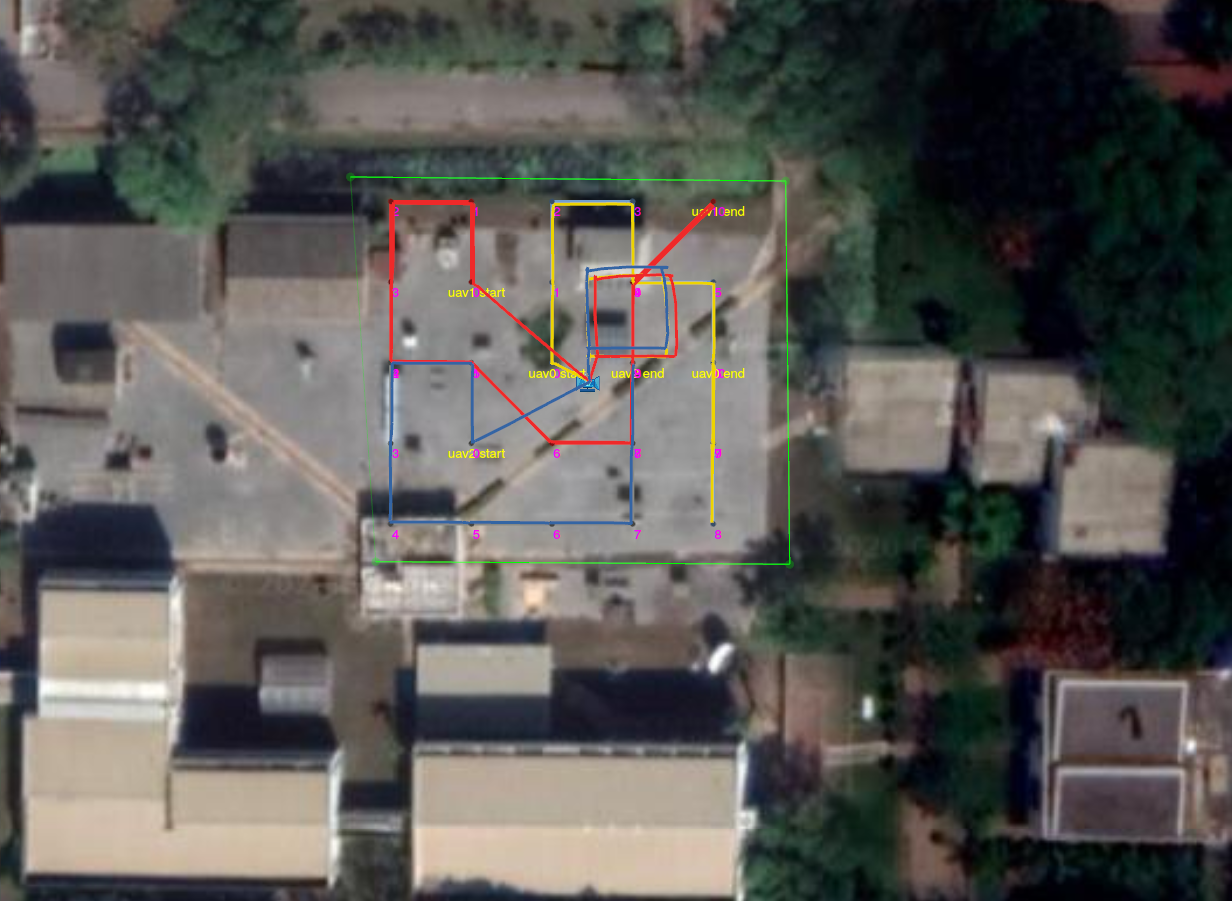
\includegraphics[width=5in]{figures/experiment/simulated-path}
	\label{fig:simulated-path}
\end{figure}

\subsection{Image Acquisition}
Thirty images were acquired from the 3 drones in real time. The images are captured with gst (gstreamer) camera plugin for gazebo and do not have any distortion. The captured images are shown in Figure~\ref{fig:simulated-images}. The position of images as described by the EXIF tag is shown in Figure~\ref{fig:simulated-images-position}.
\begin{figure}
	\centering
	\caption[The images captures in real-time during simulation.]{\small The images captured in real-time during simulation.} 
	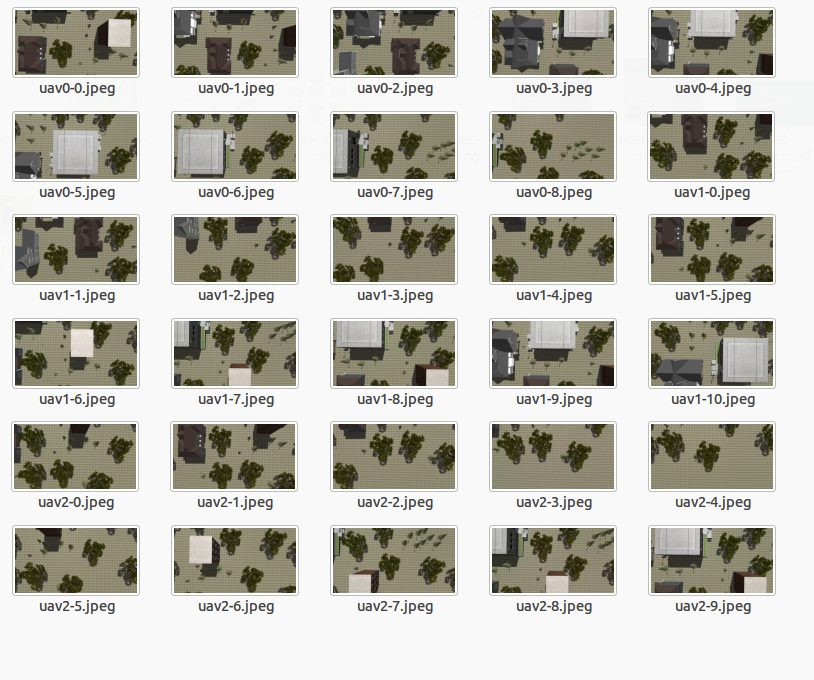
\includegraphics[width=6in]{figures/experiment/simulated-images}
	\label{fig:simulated-images}
\end{figure}
\begin{figure}
	\centering
	\caption[The GPS location of the images captured during simulation.]{\small The GPS location of the images captured during simulation.} 
	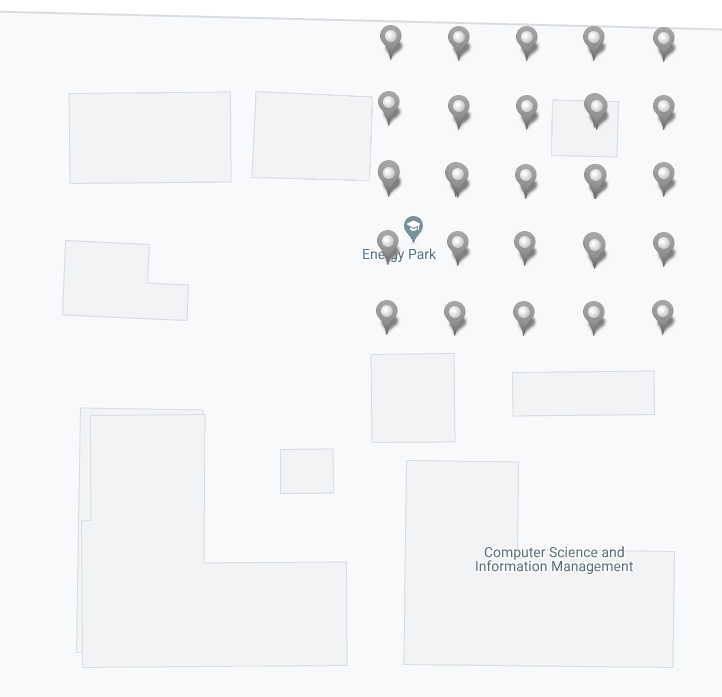
\includegraphics[width=5in]{figures/experiment/simulated-image-position}
	\label{fig:simulated-images-position}
\end{figure}

\subsection{Results}
The network traffic and the ODM outputs are analyzed for the simulation.

\subsubsection{Network Properties}
The traffic in the simulated network is captured in pcap format and wireshark is used to analyse the traffic. The distribution packet size is given in Table~\ref{tab:packet-size}. The ratio of protocol in the network is given in Table~\ref{tab:packet-protocol}. The amount of traffic generated by pegasus system for control and image messages are given in Table~\ref{tab:traffic-generation}.

\begin{table}[t]
	\caption[Distribution of packet size in the simulated network.]{\small Distribution of packet size in the simulated network.}
	\begin{center}
		\begin{tabular}{llllll}
			\hline Packet Lengths   & Count  & Average Length & Min Length & Max Length & Percent \\ \hline \hline
			All              & 217479 & 166.18         & 14         & 1046       & 100\%   \\
			0-19             & 45799  & 14             & 14         & 14         & 21.06\% \\
			20-39            & 0      & -              & -          & -          & 0.00\%  \\
			40-79            & 68814  & 74.15          & 45         & 78         & 31.64\% \\
			80-159           & 82414  & 115.43         & 80         & 122        & 37.90\% \\
			160-319          & 122    & 182.59         & 175        & 270        & 0.06\%  \\
			320-639          & 566    & 343.41         & 323        & 568        & 0.26\%  \\
			640-1279         & 19764  & 1045.66        & 669        & 1046       & 9.09\%  \\
			1280-2559        & 0      & -              & -          & -          & 0.00\%  \\
			2560-5119        & 0      & -              & -          & -          & 0.00\%  \\
			5120 and greater & 0      & -              & -          & -          & 0.00\% \\  \hline
		\end{tabular}
	\end{center}
	\label{tab:packet-size}
\end{table}

\begin{table}[t]
	\caption[Protocol distribution in the simulated network.]{\small Protocol distribution in the simulated network.}
	\begin{center}
		\begin{tabular}{lllll}
			\hline Protocol                              & Percent Packets & Packets & Percent Bytes & Bytes    \\ \hline \hline
			Malformed Packet                      & 0.15            & 335     & 0.000         & 0        \\
			Logical-Link Control                  & 47.33           & 102928  & 73.296        & 26488790 \\
			Internet Protocol Version 4           & 47.29           & 102836  & 5.691         & 2056720  \\
			User Datagram Protocol                & 47.29           & 102836  & 2.276         & 822688   \\
			Real-time Transport Control  & 0.02            & 36      & 0.065         & 23472    \\
			Optimized Link State Routing  & 27.18           & 59120   & 7.194         & 2599896  \\
			Data                                  & 20.07           & 43647   & 54.640        & 19746698 \\
			Address Resolution Protocol           & 0.04            & 92      & 0.007         & 2576     \\ \hline
		\end{tabular}
	\end{center}
	\label{tab:packet-protocol}
\end{table}

\begin{table}[t]
	\caption[ Traffic generated by pegasus system.]{\small Traffic generated by pegasus system.}
	\begin{center}
		\begin{tabular}{lllllll}
			\hline Address A & Port A & Address B & Port B & Packets & Bytes   & Type   \\ \hline \hline
			10.1.3.2  & 5444   & 10.1.3.1  & 3444   & 517     & 105753  & motion \\
			10.1.3.2  & 7300   & 10.1.3.1  & 7200   & 12122   & 6619985 & Image  \\
			10.1.3.3  & 5445   & 10.1.3.1  & 3445   & 390     & 79439   & motion \\
			10.1.3.3  & 7301   & 10.1.3.1  & 7201   & 15829   & 8519059 & Image  \\
			10.1.3.4  & 5446   & 10.1.3.1  & 3446   & 464     & 95158   & motion \\
			10.1.3.4  & 7302   & 10.1.3.1  & 7202   & 14394   & 7762232 & Image  \\ \hline
		\end{tabular}
	\end{center}
	\label{tab:traffic-generation}
\end{table}

\subsubsection{Map building}
The images do not have distortion, hence they are directly processed using WebODM.
\begin{itemize}
	\item Figure~\ref{fig:orthophoto-simulated} shows the orthophoto of the region of interest.
	\item Figure~\ref{fig:simulated-pointcloud} shows the point cloud of the region of interest.
	\item Figure~\ref{fig:textured-map-simulated} shows the textured model of the region of interest.
	\item Figure~\ref{fig:simulated-camera-position} shows the camera position as determined by ODM of the region of interest.
\end{itemize}

\begin{figure}
	\centering
	\caption[Orthophoto of simulated region of interest.]{\small Orthophoto of simulated region of interest.} 
	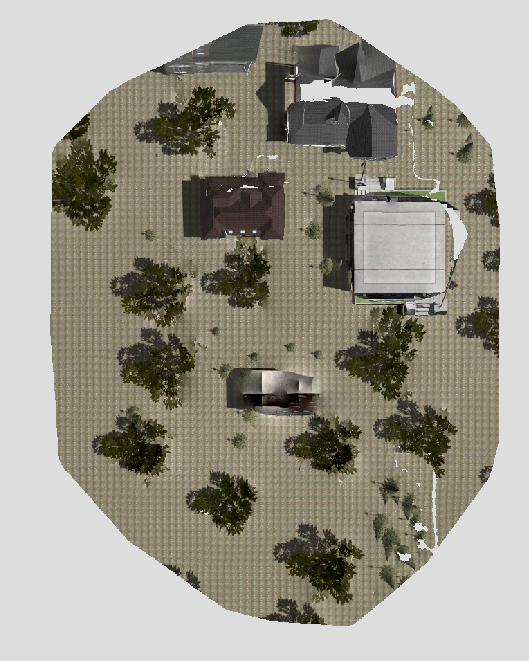
\includegraphics[width=5in]{figures/experiment/orthophoto-simulated}
	\label{fig:orthophoto-simulated}
\end{figure}

\begin{figure}
	\centering
	\caption[Point cloud of simulated region of interest.]{\small Point cloud of simulated region of interest.} 
	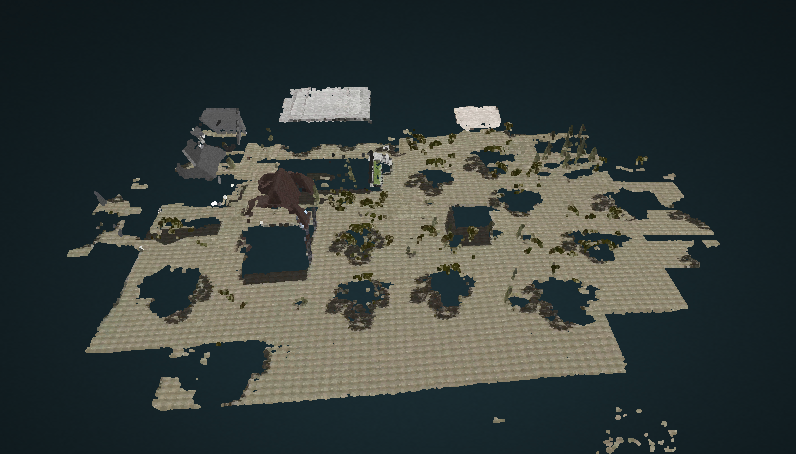
\includegraphics[width=5in]{figures/experiment/simulated-pointcould}
	\label{fig:simulated-pointcloud}
\end{figure}

\begin{figure}
	\centering
	\caption[Textured mesh of simulated region of interest.]{\small Textured mesh of simulated region of interest.} 
	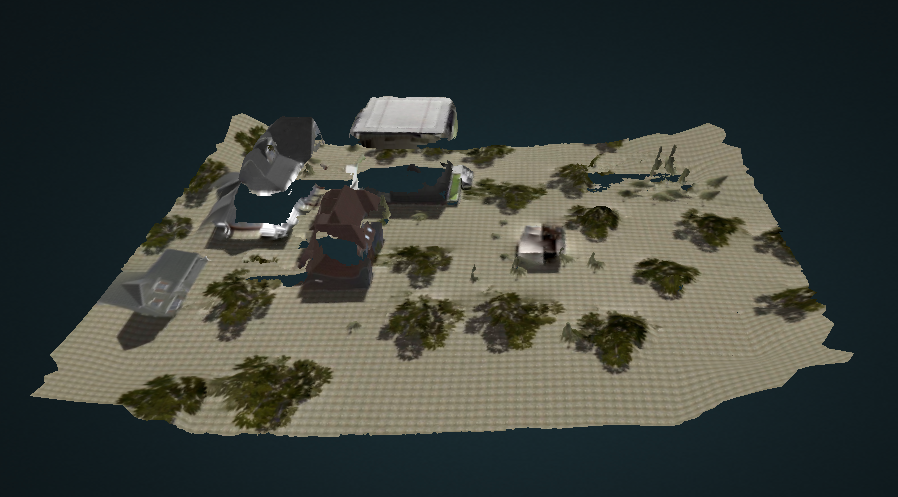
\includegraphics[width=5in]{figures/experiment/textured-simulated}
	\label{fig:textured-map-simulated}
\end{figure}

\begin{figure}
	\centering
	\caption[Position of simulated camera calculated by ODM.]{\small Position of simulated camera calculated by ODM.} 
	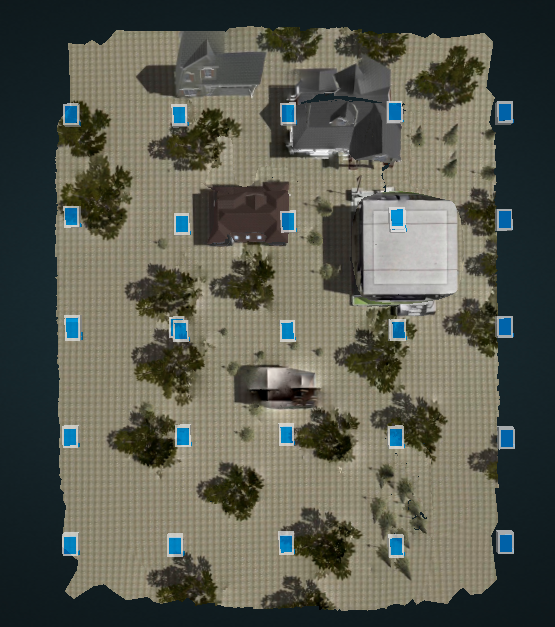
\includegraphics[width=5in]{figures/experiment/simulated-camera}
	\label{fig:simulated-camera-position}
\end{figure}

\section{Chapter Summary}
All chapters except Chapter 1 must include an introductory paragraph/s and a chapter summary.


\FloatBarrier